\documentclass[journal,10pt]{IEEEtran}

\usepackage{amsmath,amssymb,mathtools}
\usepackage{amsthm}
\usepackage{booktabs}
\usepackage{array}
\usepackage{algorithm2e}
\usepackage{cite}
\usepackage[hidelinks]{hyperref}
\usepackage{xcolor}

\newcommand{\RR}{\mathbb{R}}
\newcommand{\CC}{\mathbb{C}}
\newcommand{\ac}{\mathrm{ac}}
\newcommand{\dc}{\mathrm{dc}}
\newcommand{\gfm}{\mathrm{GFM}}
\newcommand{\vsc}{\mathrm{VSC}}
\newcommand{\diag}{\operatorname{diag}}
\newcommand{\clip}{\operatorname{clip}}
\newcommand{\median}{\operatorname{mid}}
\newcommand{\nnz}{\operatorname{nnz}}
\newcommand{\Bsub}{\partial_B}
\newcommand{\Clarke}{\partial_C}

\newtheorem{assumption}{Assumption}
\newtheorem{proposition}{Proposition}
\newtheorem{theorem}{Theorem}
\newtheorem{corollary}{Corollary}
\newtheorem{remark}{Remark}

\title{Structure-Preserving Semismooth Newton Method for Large-Scale Hybrid AC/DC Power Flow With Converter Limit-Induced Mode Switching}

\author{Tianyang~Zhao}

\markboth{Initial Research Manuscript}%
{Zhao: Structure-Preserving Semismooth Newton Hybrid AC/DC Power Flow}

\begin{document}
\maketitle

\begin{abstract}
Converter-dominated hybrid ac/dc grids exhibit operating-mode changes when
voltage-source converters reach ac-current, active-power, reactive-power, or
dc-voltage-control limits. Conventional power-flow implementations commonly
handle these events by external if--else switching, which changes equation
semantics and may rebuild the sparse Newton system. This paper develops a
fixed-dimension complementarity formulation and a structure-preserving
semismooth Newton method for balanced positive-sequence hybrid ac/dc power
flow. Each limited converter owns six explicit local variables representing
ac active and reactive power, dc power, internal-voltage components, and a
complementarity multiplier. The formulation covers current-magnitude scaling,
active- or reactive-power priority, saturated dc-voltage droop, and a
grid-forming Norton source behind virtual impedance. An exact local-block
Schur elimination removes the converter variables before sparse network
factorization without forming dense inverses. Local reciprocal-condition and
reduced/full-system backward-error certificates guard every Schur step and
trigger a complete sparse-LU fallback when necessary. Conditional local
superlinear and quadratic convergence results are stated under BD-regularity
and strong semismoothness, while runtime diagnostics deliberately certify only
the selected generalized-Jacobian element. Preliminary production results on
hybridized case300 and ACTIVSg2000 systems show exact full/Schur root agreement
within $10^{-8}$ p.u. The reduced formulation decreases dimension from 4054
to 4006 on ACTIVSg2000 and lowers median linear-solve and end-to-end times by
14.0\% and 12.5\%, respectively. The same method is exercised under
simultaneous converter limiting, degenerate intersections, weak grids,
infeasible operating points, grid-forming islands, OpenDSS circuit replay,
optimal-power-flow replay, and transient initialization.
\end{abstract}

\begin{IEEEkeywords}
Complementarity constraints, grid-forming converter, hybrid ac/dc power flow,
mode switching, semismooth Newton method, Schur complement, voltage-source
converter.
\end{IEEEkeywords}

\section{Introduction}\label{sec:introduction}

\IEEEPARstart{H}{ybrid} ac/dc grids are increasingly operated through
voltage-source converters rather than through passive interfaces. Multi-terminal
dc links, offshore-wind collection systems, converter-interfaced generation,
and grid-forming resources make converter control limits part of the network
equilibrium itself. A converter may regulate active and reactive power, dc
voltage, or an internal ac voltage during normal operation, but semiconductor
current limits remain hard physical constraints. Once a limit becomes active,
the unconstrained command can no longer be maintained and the steady or
quasi-steady operating point changes control regime.

This limit-induced mode switching is more involved than the classical
generator PV/PQ transition. A converter can encounter an ac-current disk, a dc
power bound, saturated dc-voltage droop, and a selected priority between active
and reactive current. For a grid-forming converter, current limiting also
modifies the relation between the internal voltage source and the terminal
voltage. Consequently, a post-limit equilibrium may require explicit internal
voltage and current variables rather than a bus-level net-injection correction.
These issues are especially important in islanded networks, where a fixed GFM
internal phasor can provide the absolute angle reference without manufacturing
a terminal slack bus.

Unified hybrid ac/dc power-flow methods have improved the treatment of ac
networks, dc networks, and converter coupling
\cite{javid2023unified,sun2024mdhem,pompodakis2021generic}. In parallel, GFM
control and fault-current-limiting studies have clarified how a voltage-source
behavior is modified by current constraints
\cite{rocabert2012microgrid,baeckeland2022stationary}. Most power-flow
implementations nevertheless retain an external engineering loop of the form
``solve, inspect a limit, switch the device model, and solve again.'' This
approach is practical for isolated limits, but its equation dimension,
variable semantics, and sparse pattern may depend on the switching sequence.
Simultaneous activation, priority ties, and return switching can also make the
final result sensitive to implementation order.

Complementarity equations provide a fixed-dimensional alternative. A limit
and its multiplier are solved together, allowing the inactive and active
regimes to be represented by one nonsmooth system
\cite{facchinei2003complementarity,fischer1992newton}. Semismooth Newton
methods can then achieve fast local convergence without enumerating all mode
combinations \cite{qi1993nonsmooth}. Their use in a production hybrid ac/dc
solver, however, raises three additional questions. First, the converter must
own explicit local variables so that device equations and result certificates
do not have to be reconstructed from aggregated bus injections. Second, the
fixed equation layout must translate into a measurable sparse-linear-algebra
advantage rather than only a software convenience. Third, local convergence
claims must distinguish a numerically accepted generalized-Jacobian element
from the stronger BD-regularity condition over the B-subdifferential.

This paper addresses these questions through a balanced positive-sequence
hybrid ac/dc formulation with explicit converter blocks. Each supported VSC
owns the local state
\begin{equation}
 z_c=(P_{\ac,c},Q_{\ac,c},P_{\dc,c},E_{r,c},E_{i,c},\lambda_c),
 \label{eq:local-state-intro}
\end{equation}
where the internal-voltage slots are active for GFM operation and are fixed by
identity equations for power-port modes. Current-magnitude scaling uses a
Fischer--Burmeister equation. Active- and reactive-power priorities use nested
median projections. Vdc-Q operation includes a saturated dc-voltage droop
command, and GFM operation uses an internal voltage behind virtual impedance.
All equations remain present across limit activation.

The main contributions are as follows.

\begin{enumerate}
  \item A unified fixed-dimensional converter-limit model is developed for
  PQ, Vdc-Q, and GFM operation. It combines the ac-current disk, magnitude or
  P/Q priority, converter energy balance, saturated dc-voltage droop, and GFM
  Norton equations while preserving stable device identity and explicit local
  result variables.

  \item A production semismooth Newton method is formulated with analytic
  network/local generalized Jacobians. Exact Fischer--Burmeister and median
  equations define the reported root; optional Kanzow/CHKS smoothing provides
  a fixed-pattern continuation for difficult degenerate points. A full sparse
  Newton fallback remains available at every iteration.

  \item An exact local-block Schur method eliminates all six-state converter
  blocks before network factorization. The method has $O(m)$ local dense work
  for $m$ converters, removes exactly $6m$ unknowns, and reduces the assembled
  structural nonzeros by at least $48m$ under the stated three-port coupling
  pattern. Local reciprocal-condition and normwise backward-error tests guard
  the reduced and reconstructed full steps.

  \item The convergence statement separates mathematics from runtime
  evidence. BD-regularity plus semismoothness yields local superlinear
  convergence, and strong semismoothness yields the standard quadratic rate.
  Runtime certificates establish nonsingularity and backward stability only
  for the selected generalized-Jacobian element; they are not presented as a
  proof over every element of the B-subdifferential.

  \item The implementation is exercised through registered production tests,
  OpenDSS circuit validation, OPF-to-PF replay, transient Norton initialization,
  simultaneous limits, weak-grid and infeasible cases, GFM islands, and real
  hybrid case300/ACTIVSg2000 benchmarks. The preliminary results also retain a
  negative small-system performance result, which motivates an explicit and
  configurable production admission rule.
\end{enumerate}

Figure~\ref{fig:problem-method} summarizes the problem, model ownership, and
solver structure. The central distinction is that limit activation changes
residual values and generalized derivatives, but not the converter state,
equation coordinates, or sparse ownership map.

\begin{figure*}[t]
\centering
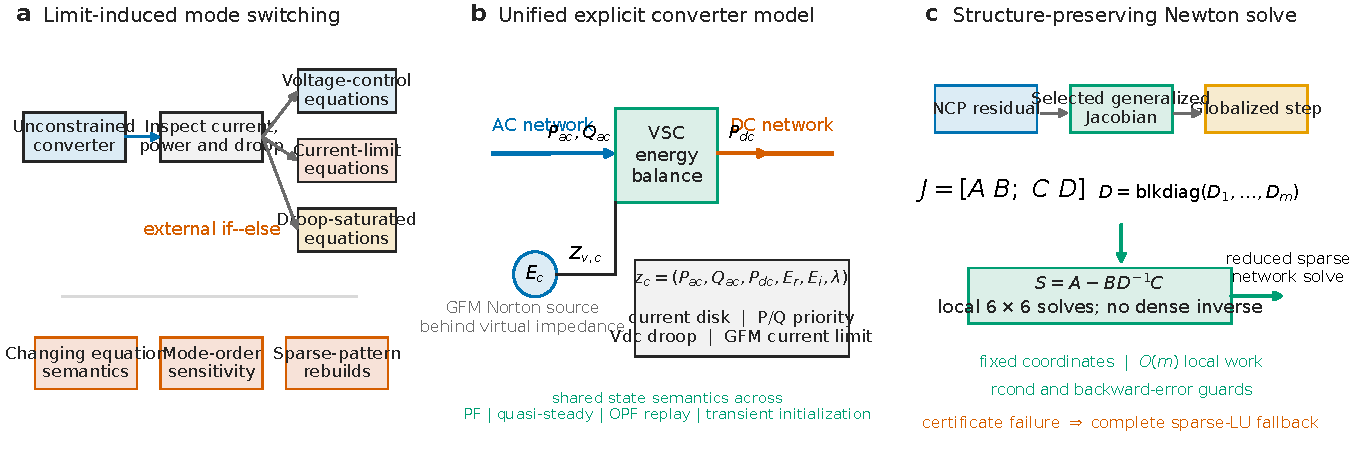
\includegraphics[width=\textwidth]{figures/problem_method_overview.pdf}
\caption{From limit-induced switching to the proposed fixed-dimensional
framework. (a) External mode switching can change equation semantics and
sparse structure. (b) Each VSC instead owns one explicit six-state block,
including the GFM internal voltage behind virtual impedance. (c) The resulting
fixed generalized-Jacobian pattern supports certified local-block Schur
elimination with complete sparse-LU fallback.}
\label{fig:problem-method}
\end{figure*}

The paper is organized as follows. Section~\ref{sec:model} defines the network
and converter equations. Section~\ref{sec:ssn} presents the semismooth Newton
method. Section~\ref{sec:schur} derives the exact local-block Schur elimination
and its cost. Section~\ref{sec:convergence} states the regularity and local-rate
conditions. Section~\ref{sec:preliminary} reports the current production
evidence and its limitations.

\section{Hybrid AC/DC and Converter-Limit Model}\label{sec:model}

\subsection{Network variables and nodal balances}

Let $\mathcal N_{\ac}$ and $\mathcal N_{\dc}$ denote the energized ac and dc
buses, and let $\mathcal C$ denote the supported limited VSCs. The network
state is
\begin{equation}
 x=(\theta,V,V_{\dc}),
\end{equation}
with only the coordinates required by the selected bus equations retained.
In a conventional grid-connected component, one terminal angle is omitted or
fixed. In a slackless GFM island, all terminal voltage magnitudes and angles
remain variables; a fixed internal GFM phasor supplies the absolute reference
through the device equation.

For ac bus $i$, the calculated complex injection is
\begin{equation}
 S_i^{\mathrm{net}}(V,\theta)
 =V_i e^{\mathrm j\theta_i}
  \overline{\sum_{k\in\mathcal N_{\ac}}
  Y_{ik}V_k e^{\mathrm j\theta_k}}.
\end{equation}
The active- and reactive-power residuals are written in the production
``specified minus calculated'' convention,
\begin{subequations}\label{eq:ac-balances}
\begin{align}
 F_{P,i} &= P_i^{\mathrm{spec}}(x,z)-\Re(S_i^{\mathrm{net}}),\\
 F_{Q,i} &= Q_i^{\mathrm{spec}}(x,z)-\Im(S_i^{\mathrm{net}}).
\end{align}
\end{subequations}
For dc bus $j$, with conductance matrix $G_{\dc}$,
\begin{equation}
 F_{\dc,j}=P_{\dc,j}^{\mathrm{spec}}(x,z)
 -V_{\dc,j}(G_{\dc}V_{\dc})_j.
 \label{eq:dc-balance}
\end{equation}
Each converter contributes its explicit $(P_{\ac,c},Q_{\ac,c},P_{\dc,c})$
directly to the corresponding nodal balances. This ownership is important:
converter power, limit activity, and internal-voltage results are solver
variables and certificates, not values inferred after convergence from a bus
net injection.

\subsection{Fixed local converter state}

Every $c\in\mathcal C$ owns the six-state vector in
\eqref{eq:local-state-intro}. The complete nonlinear system is
\begin{equation}
 H(w)=0,\qquad
 w=(x,z_1,\ldots,z_m),\quad m=|\mathcal C|,
 \label{eq:complete-system}
\end{equation}
where $H$ stacks the network balances and six local equations per converter.
The local state has one meaning across steady power flow, quasi-steady replay,
OPF post-processing, and transient initialization. For non-GFM power-port
modes, $E_{r,c}=E_{i,c}=0$ are identity equations; the slots are retained so
the dimension and sparse coordinates do not change with control role.

\subsection{Power command and dc-voltage droop saturation}

For PQ operation,
\begin{equation}
 P_c^{\mathrm{ref}}=P_c^{\mathrm{set}},\qquad
 Q_c^{\mathrm{ref}}=Q_c^{\mathrm{set}}.
\end{equation}
For Vdc-Q operation, the active-power command is
\begin{subequations}\label{eq:vdc-droop}
\begin{align}
 P_c^{\mathrm{raw}}
 &=k_{v,c}\left(V_{\dc,c}^{2}-(V_{\dc,c}^{\mathrm{set}})^2\right),\\
 P_c^{\mathrm{ref}}
 &=\clip(P_c^{\mathrm{raw}},P_c^{\min},P_c^{\max}),\\
 Q_c^{\mathrm{ref}}&=Q_c^{\mathrm{set}}.
\end{align}
\end{subequations}
Inside the open unsaturated interval,
$\partial P_c^{\mathrm{ref}}/\partial V_{\dc,c}=2k_{v,c}V_{\dc,c}$;
outside it the derivative is zero. The power bounds are therefore represented
inside the local equations rather than through an external mode switch.

\subsection{Current disk and power-port priorities}

For terminal voltage magnitude $V_c$ and current limit $I_c^{\max}$, define
\begin{equation}
 R_c=V_c I_c^{\max},\qquad
 g_c=R_c^2-P_{\ac,c}^2-Q_{\ac,c}^2.
 \label{eq:current-disk}
\end{equation}
The magnitude-priority model radially scales the requested complex power:
\begin{subequations}\label{eq:magnitude-priority}
\begin{align}
 (1+\lambda_c)P_{\ac,c}-P_c^{\mathrm{ref}}&=0,\\
 (1+\lambda_c)Q_{\ac,c}-Q_c^{\mathrm{ref}}&=0,\\
 \phi_{\mathrm{FB}}(\lambda_c,g_c)&=0,
\end{align}
\end{subequations}
where
\begin{equation}
 \phi_{\mathrm{FB}}(a,b)=\sqrt{a^2+b^2}-a-b.
 \label{eq:fb}
\end{equation}
Equation~\eqref{eq:fb} is zero exactly when
$a\ge0$, $b\ge0$, and $ab=0$.

For P-first and Q-first operation, define the median projection residual
\begin{equation}
 \mathcal M(y;r,\ell,u)
 =\max\!\left(\min(y-r,y-\ell),y-u\right).
 \label{eq:median}
\end{equation}
The equation $\mathcal M=0$ returns the reference when it is feasible and the
nearest bound otherwise. P-first operation is
\begin{subequations}\label{eq:p-first}
\begin{align}
 \mathcal M(P_{\ac,c};P_c^{\mathrm{ref}},-R_c,R_c)&=0,\\
 R_{Q,c}&=\sqrt{\max(0,R_c^2-P_{\ac,c}^2)},\\
 \mathcal M(Q_{\ac,c};Q_c^{\mathrm{ref}},-R_{Q,c},R_{Q,c})&=0,\\
 \lambda_c&=0.
\end{align}
\end{subequations}
Q-first operation exchanges $P$ and $Q$ in \eqref{eq:p-first}. A finite
selected generalized derivative is used when the remaining radius is zero.

Figure~\ref{fig:priority-geometry} shows the geometric distinction among the
three policies for one normalized infeasible request. Magnitude limiting moves
radially to the current circle. P-first retains the feasible active component
before assigning the remaining reactive radius, whereas Q-first performs the
dual construction. The figure is an equation-level illustration; measured
production results are reported separately in Section~\ref{sec:preliminary}.

\begin{figure*}[t]
\centering
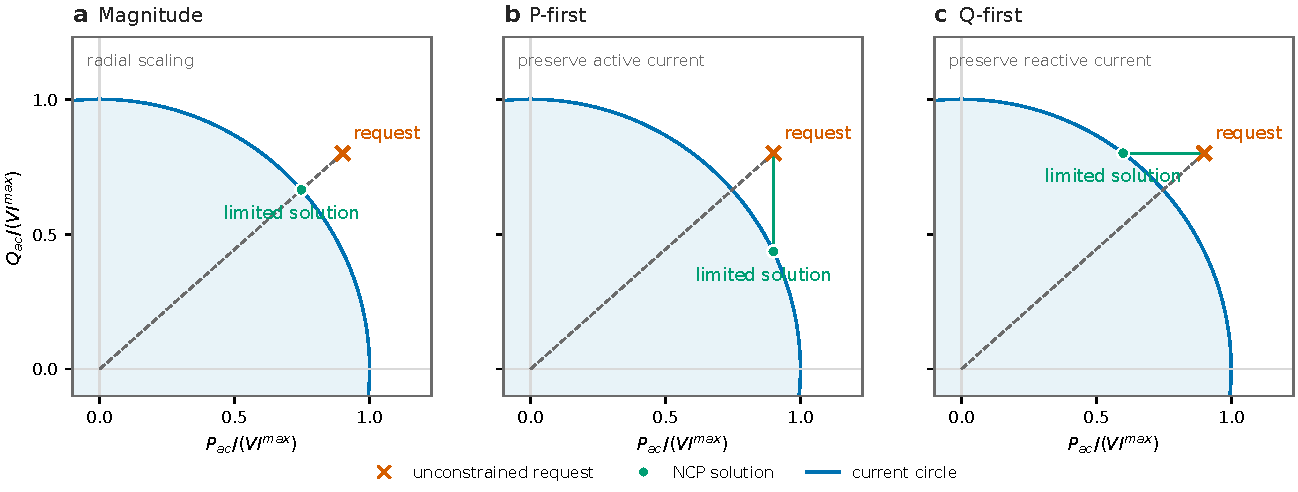
\includegraphics[width=0.92\textwidth]{figures/priority_geometry.pdf}
\caption{Normalized current-circle geometry for the common infeasible request
$(P^{\mathrm{ref}},Q^{\mathrm{ref}})/(VI^{\max})=(0.9,0.8)$. The orange cross
is the unconstrained command and the green point is the NCP solution.
(a) Magnitude priority scales both components radially. (b) P-first preserves
active current and clips reactive current to the remaining radius. (c) Q-first
preserves reactive current and clips active current.}
\label{fig:priority-geometry}
\end{figure*}

All power-port priorities close converter energy balance through
\begin{equation}
 P_{\dc,c}+P_{\ac,c}
 +P_c^{\mathrm{loss}}(P_{\ac,c},V_{\dc,c})=0,
 \label{eq:energy-balance}
\end{equation}
with analytic derivatives from the selected production loss model.

\subsection{Grid-forming Norton equation family}

Let
\begin{equation}
 \mathcal V_c=V_c e^{\mathrm j\theta_c},\quad
 E_c=E_{r,c}+\mathrm jE_{i,c},\quad
 Z_{v,c}=R_{v,c}+\mathrm jX_{v,c}.
\end{equation}
The converter current and terminal power are
\begin{equation}
 I_c=\frac{E_c-\mathcal V_c}{Z_{v,c}},\qquad
 S_{\ac,c}=\mathcal V_c\overline{I_c}
 =P_{\ac,c}+\mathrm jQ_{\ac,c}.
 \label{eq:gfm-port}
\end{equation}
Thus the first two local equations enforce the real and imaginary parts of
\eqref{eq:gfm-port}, and \eqref{eq:energy-balance} supplies the third.

For magnitude limiting, let $E_c^0$ be the authored internal-voltage reference.
The remaining equations are
\begin{subequations}\label{eq:gfm-magnitude}
\begin{align}
 (1+\lambda_c)(E_c-\mathcal V_c)
 -(E_c^0-\mathcal V_c)&=0,\\
 \phi_{\mathrm{FB}}\!\left(
 \lambda_c,(I_c^{\max})^2-|I_c|^2\right)&=0.
\end{align}
\end{subequations}
The complex equation in \eqref{eq:gfm-magnitude} supplies two real rows. It can
be interpreted as an implicit increase in the virtual impedance when the
current circle becomes active.

For P-first and Q-first GFM limiting, $I_c$ and the unconstrained current
$I_c^0=(E_c^0-\mathcal V_c)/Z_{v,c}$ are rotated into the terminal-voltage synchronous
frame. The primary current component is projected onto
$[-I_c^{\max},I_c^{\max}]$ using \eqref{eq:median}; the secondary component is
projected onto its remaining circular radius. The unused multiplier is fixed
by $\lambda_c=0$. This construction preserves the same six rows and variables
for all three priorities.

\subsection{Model scope}

The equations describe a balanced positive-sequence steady or quasi-steady
operating point after limit activation. They do not represent PWM switching,
the fast current-control transient, or EMT fault dynamics. A GFM terminal in a
slackless island retains its terminal $V/\theta$ variables and both nodal power
balances. The authored internal phasor $E_c^0$ breaks the global rotational
null mode through \eqref{eq:gfm-port}; no artificial terminal slack is added.
Multiple fixed Norton sources can coexist, with power sharing and circulating
power determined by their phasors and virtual impedances.

\section{Structure-Preserving Semismooth Newton Method}\label{sec:ssn}

\subsection{Nonsmooth residual and generalized Jacobian}

Let $H:\RR^n\rightarrow\RR^n$ denote the complete residual in
\eqref{eq:complete-system}. Smooth ac/dc network equations and converter loss
functions are combined with the locally Lipschitz Fischer--Burmeister and
median maps. The resulting $H$ is differentiable away from switching ties and
semismooth at the ties under the standard NCP construction
\cite{facchinei2003complementarity,qi1993nonsmooth}.

At iteration $k$, one element
\begin{equation}
 J_k\in\Bsub H(w_k)
 \label{eq:selected-jacobian}
\end{equation}
is assembled analytically. The network part follows the production convention
$J_{\mathrm{net}}=\partial(\mathrm{calculated}-\mathrm{specified})/\partial x$
with right-hand side equal to the network mismatch. Local converter rows store
the conventional derivative of their zero residual and use right-hand side
$-H_c$. This sign split is resolved during assembly into one linear system
\begin{equation}
 J_k d_k=-H(w_k).
 \label{eq:newton-step}
\end{equation}

The exact Fischer--Burmeister map is not regularized by a hidden epsilon. At
the biactive origin, the implementation selects the symmetric Clarke element
\begin{equation}
 \left(\frac{1}{\sqrt 2}-1,
       \frac{1}{\sqrt 2}-1\right)\in
 \Clarke\phi_{\mathrm{FB}}(0,0).
 \label{eq:fb-origin}
\end{equation}
For the median map, the active branch determines the derivative; equal
branches use an equal-weight finite selection. This policy makes the selected
matrix deterministic while retaining the fixed equation layout.

\subsection{Optional smooth continuation}

Degenerate intersections may cause an abrupt change in the selected
generalized Jacobian. The optional continuation replaces
\eqref{eq:fb} with the Kanzow smoothing
\begin{equation}
 \phi_{\mu}(a,b)
 =\sqrt{a^2+b^2+2\mu^2}-a-b,
 \qquad \mu>0,
 \label{eq:smooth-fb}
\end{equation}
and replaces nested min/max operations in \eqref{eq:median} with the
Chen--Harker--Kanzow--Smale smooth composition
\cite{kanzow1996continuation}. The parameter is reduced from $\mu_0$ to
$\mu_{\min}$ using a coarse/fine multiplicative schedule. After each reduction,
the residual and Jacobian are reassembled at the unchanged state. Only matrix
values change; variable order and sparse coordinates do not.

The reported operating point is always re-evaluated with $\mu=0$. Thus a small
smooth surrogate residual is not reported as an exact complementarity
certificate. Smooth continuation is a globalization aid, not a change to the
target physical model.

\subsection{Globalized iteration}

The production method combines the local semismooth step with residual and
variable scaling, a nonmonotone line search, and fail-closed fallbacks. Let
$D_F$ and $D_w$ denote residual and variable scaling matrices. The scaled
linear system is
\begin{equation}
 (D_FJ_kD_w^{-1})\widehat d_k=-D_FH(w_k),\qquad
 d_k=D_w^{-1}\widehat d_k.
 \label{eq:scaled-newton}
\end{equation}
The line search accepts $w_{k+1}=w_k+\alpha_k d_k$ when the merit function
$\Psi(w)=\tfrac12\|D_FH(w)\|_2^2$ satisfies a nonmonotone sufficient-decrease
test. Trust-region, pseudo-transient, active-set-seeded, and homotopy paths
remain external global safeguards; none changes the fixed local VSC state.

\begin{algorithm}[t]
\caption{Structure-preserving semismooth Newton solve}
\label{alg:ssn}
\KwIn{Hybrid system data, initial state $w_0$, tolerances, $\mu_0$}
Build the network and six-state-per-VSC sparse pattern once\;
Analyze the full and admissible reduced patterns once\;
\For{$k=0,1,\ldots,k_{\max}-1$}{
  Evaluate exact or $\mu_k$-smoothed $H(w_k)$\;
  \If{the exact target residual satisfies the stopping test}{return certified root\;}
  Assemble one selected analytic generalized Jacobian $J_k$\;
  Attempt the certified local-block Schur step\;
  \If{a Schur certificate fails}{solve the complete sparse system\;}
  Apply scaling and the globalized step acceptance rule\;
  \If{the smooth residual has decreased sufficiently and $\mu_k>\mu_{\min}$}{
    reduce $\mu_k$ and reassemble at the accepted state\;
  }
}
Return an explicit nonconvergence or infeasibility diagnosis\;
\end{algorithm}

\subsection{Structure preservation}

Each admitted converter always contributes six rows and six columns. A limit
activation, priority tie, or droop saturation modifies residual and Jacobian
values but not coordinates. Therefore the matrix memory layout, device-to-row
mapping, symbolic analysis, and result index remain stable. This property
removes repeated structural allocation and is also the prerequisite for the
local Schur method in Section~\ref{sec:schur}.

The fixed pattern does not imply that every numerical factorization can reuse
the same pivots. Numeric-only KLU refactorization is attempted only after a
previous factorization and is guarded by a normwise backward-error test. A
failed refactorization or an inaccurate solution triggers fresh pivoting.

\section{Exact Local VSC-Block Schur Elimination}\label{sec:schur}

\subsection{Block structure}

Order the Newton variables so that all network variables precede the local VSC
states. The selected generalized Jacobian and right-hand side are
\begin{equation}
 \begin{bmatrix}A&B\\C&D\end{bmatrix}
 \begin{bmatrix}d_x\\d_z\end{bmatrix}
 =\begin{bmatrix}r_x\\r_z\end{bmatrix},
 \qquad
 D=\diag(D_1,\ldots,D_m),
 \label{eq:block-newton}
\end{equation}
where $D_c\in\RR^{6\times6}$. Converter $c$ couples only to its terminal
angle, terminal voltage magnitude, and dc voltage. Conversely, its explicit
power variables enter only the terminal ac-P, ac-Q, and dc-P network rows.

When every $D_c$ is nonsingular, block Gaussian elimination gives
\begin{subequations}\label{eq:schur-system}
\begin{align}
 S&=A-BD^{-1}C,\\
 \widehat r_x&=r_x-BD^{-1}r_z,\\
 Sd_x&=\widehat r_x,\\
 d_z&=D^{-1}(r_z-Cd_x).
\end{align}
\end{subequations}
The implementation does not form $D_c^{-1}$. One dense full-pivoting
factorization of each $6\times6$ block solves the four right-hand sides
$[C_c,r_c]$. The resulting $3\times3$ update is scattered into precomputed
coordinates of the reduced sparse matrix.

\begin{proposition}[Algebraic equivalence]\label{prop:schur-equivalence}
Suppose every $D_c$ and the Schur complement $S$ in
\eqref{eq:schur-system} are nonsingular. Then the reduced solve and back
substitution produce the unique solution of the complete system
\eqref{eq:block-newton}.
\end{proposition}

\begin{proof}
The second block row gives $d_z=D^{-1}(r_z-Cd_x)$. Substitution into the first
block row yields $Sd_x=\widehat r_x$. Nonsingularity gives a unique $d_x$ and
then a unique $d_z$. Direct substitution verifies both block rows
\cite{golub2013matrix}.
\end{proof}

\subsection{Fixed reduced pattern}

The network submatrix $A$ retains its ordinary sparse coordinates. Each local
block has at most three coupled network rows and three coupled network columns,
so $BD^{-1}C$ modifies at most nine network coordinates per converter. Those
coordinates are inserted into the reduced pattern during initialization, even
when their current numerical value is zero. Consequently, switching activity
does not require a new symbolic analysis.

For local state size $s=6$ and network coupling width $c\le3$, the dense local
work is
\begin{equation}
 O\!\left(ms^3+ms^2(c+1)\right)=O(m).
 \label{eq:local-cost}
\end{equation}
The reduced dimension is $n_x$ rather than $n_x+6m$. In the complete fixed
pattern, one converter contributes 36 local entries, 18 local-to-network
entries, and three network-to-local entries. The reduced update adds at most
nine coordinates, so
\begin{equation}
 \nnz(J)-\nnz(S)\ge48m.
 \label{eq:nnz-bound}
\end{equation}
This is an input-pattern result, not a universal sparse-LU fill theorem. Fill,
flop count, cache behavior, and ordering remain network dependent
\cite{davis2006direct} and are measured experimentally.

\subsection{Numerical certificates and fallback}

Every local factorization reports a reciprocal condition estimate
$\rho_c$. A Schur attempt is rejected if a block is nonfinite or
\begin{equation}
 \rho_c\le\rho_{\min}.
\end{equation}
The default is
$\rho_{\min}=\sqrt{\epsilon_{\mathrm{mach}}}$, which separates the
representation scale from the requested nonlinear accuracy. This is a
conservative numerical admission test, not part of the physical model.

For a matrix $M$, right-hand side $b$, and candidate solution $y$, the
normwise backward error is evaluated as
\begin{equation}
 \eta(M,b,y)=
 \frac{\|b-My\|_{\infty}}
 {\|M\|_{\infty}\|y\|_{\infty}+\|b\|_{\infty}}.
 \label{eq:backward-error}
\end{equation}
Both the reduced solution
$\eta(S,\widehat r_x,d_x)$ and the reconstructed complete solution
$\eta(J,r,d)$ must satisfy the configured tolerance. This complete-system
check is essential because a stable reduced solve alone does not certify the
back substitution. Any local-regularity, reduced-solve, or full-step failure
returns control to the ordinary complete sparse-LU path
\cite{higham2002accuracy}.

\subsection{Production admission}

The $O(m)$ local work and certificates have a fixed latency that can dominate
a small network factorization. Therefore Schur elimination is enabled by an
empirical, configurable crossover rule rather than unconditionally. The
current production default admits the path only when the network-only Newton
dimension is at least 1000. This number is not a mathematical constant; it is a
named default derived from the fixed case300/ACTIVSg2000 protocol and can be
overridden through both the C++ and production HTTP interfaces. Setting it to
zero forces a research ablation.


\section{Regularity and Local Convergence Conditions}\label{sec:convergence}

\subsection{Semismoothness assumptions}

The following statements concern the exact target residual $H$ with $\mu=0$.

\begin{assumption}[Local model regularity]\label{ass:model-regularity}
The smooth ac/dc network, loss, and droop functions are continuously
differentiable in a neighborhood of a solution $w^*$. Terminal voltage
magnitudes and dc voltages remain inside the domain on which their physical
equations and derivatives are finite, and each admitted GFM virtual impedance
is nonzero.
\end{assumption}

\begin{assumption}[BD-regular solution]\label{ass:bd-regular}
The exact residual $H$ is semismooth at $w^*$ and every matrix
$J\in\Bsub H(w^*)$ is nonsingular.
\end{assumption}

The Fischer--Burmeister map and piecewise-affine median projection are
strongly semismooth. Their composition with the smooth network and converter
functions preserves local semismoothness under
Assumption~\ref{ass:model-regularity}. At a zero remaining-current radius, the
square-root radius in the priority model requires the explicitly selected
finite generalized branch used by the implementation. Such a selection makes
one Newton step well defined, but it does not by itself prove
Assumption~\ref{ass:bd-regular} for all neighboring selections.

\begin{theorem}[Conditional local rate]\label{thm:local-rate}
Let $w^*$ solve $H(w)=0$. Under
Assumptions~\ref{ass:model-regularity} and~\ref{ass:bd-regular}, the exact
semismooth Newton iteration \eqref{eq:newton-step}, started sufficiently close
to $w^*$ and eventually accepting the full step, is well defined and converges
superlinearly to $w^*$. If $H$ is strongly semismooth at $w^*$, the local rate
is quadratic.
\end{theorem}

\begin{proof}
The result is the standard semismooth Newton theorem applied to the square
locally Lipschitz residual $H$. BD-regularity gives uniformly bounded inverses
for the relevant B-subdifferential elements near $w^*$, while semismoothness
makes the linearization remainder $o(\|w-w^*\|)$. Strong semismoothness improves
the remainder to $O(\|w-w^*\|^2)$
\cite{qi1993nonsmooth,facchinei2003complementarity}.
\end{proof}

\subsection{Block nonsingularity condition}

\begin{proposition}[Selected-element block certificate]
Consider one selected generalized-Jacobian element $J$ partitioned as in
\eqref{eq:block-newton}. If every $D_c$ is nonsingular, then
\begin{equation}
 J\ \text{is nonsingular}
 \quad\Longleftrightarrow\quad
 S=A-BD^{-1}C\ \text{is nonsingular}.
 \label{eq:block-regularity}
\end{equation}
\end{proposition}

\begin{proof}
Block Gaussian elimination factors $J$ into nonsingular unit triangular
factors and $\diag(S,D)$. The determinant and null-space equivalence follow
immediately \cite{golub2013matrix}.
\end{proof}

Equation~\eqref{eq:block-regularity} is the theoretical basis of the runtime
Schur certificate. Local $D_c$ condition estimates, successful sparse
factorization of $S$, and the complete backward-error test provide numerical
evidence for the current selected element. They do not enumerate
$\Bsub H(w^*)$ and therefore must not be reported as a proof of BD-regularity.

\subsection{Measured local-rate diagnostics}

For accepted iterates with residual norm $r_k=\|H(w_k)\|$, the implementation
reports
\begin{equation}
 q_k^{(1)}=\frac{r_{k+1}}{r_k},\qquad
 q_k^{(2)}=\frac{r_{k+1}}{r_k^2}.
 \label{eq:rate-diagnostics}
\end{equation}
A decreasing $q_k^{(1)}$ is consistent with superlinear behavior, while a
bounded $q_k^{(2)}$ in the asymptotic regime is consistent with quadratic
behavior. These finite samples are diagnostic evidence only. Damped steps,
smoothing-parameter reductions, mode-degenerate iterations, and full-LU
fallbacks can occur outside the final local regime and should be excluded from
any empirical rate fit.

\subsection{Smoothing and globalization boundary}

The smooth continuation in \eqref{eq:smooth-fb} improves path following but
does not replace Theorem~\ref{thm:local-rate}. The final state is accepted only
after evaluation of the exact $\mu=0$ residual. Likewise, line search and
fallback scheduling improve robustness but do not establish global
convergence or uniqueness. Hybrid power-flow equations may possess both high-
and low-voltage mathematical roots, and a distant initial point may converge
to a different basin. Infeasible operating points must be reported as
nonconverged rather than converted into a plausible result.

\subsection{Numerical-policy separation}

Machine epsilon is a single read-only representation constant. Nonlinear
tolerances, the local $rcond$ threshold, the backward-error threshold, and the
Schur crossover dimension are named algorithmic policy. They are configurable
and validated separately. This prevents a hardware-scale constant from being
reused as a physical feasibility tolerance and prevents empirical admission
settings from becoming hidden universal assumptions.


\section{Preliminary Production Results}\label{sec:preliminary}

\subsection{Implementation and protocol}

The method is implemented in the production balanced Newton path of the
HySim-XJTU-HRPES C++20 codebase. All preliminary timings use an AppleClang 21
arm64 macOS Release build with KLU. The Schur benchmark parses each case once,
performs two warmups, and then executes five alternating full/Schur solves. The
reported times are medians. The benchmark forces Schur on case300 for research
ablation even though the production admission rule excludes it.

The current KLU adapter does not report factor nonzeros or factor work. Those
fields are explicitly marked unavailable; the results below report input
structural nonzeros, dimensions, iterations, and measured time without
fabricating fill statistics.

\subsection{Functional and numerical verification}

The registered VSC-limit suite passes 45 cases and 540 assertions. Its scope is
summarized in Table~\ref{tab:verification}. Analytic generalized Jacobians are
checked by finite differences away from switching ties, and the biactive
Fischer--Burmeister origin is tested without a hidden perturbation.

\begin{table*}[t]
\caption{Current verification coverage and acceptance boundaries}
\label{tab:verification}
\centering\footnotesize
\setlength{\tabcolsep}{4pt}
\begin{tabular}{p{0.19\textwidth}p{0.47\textwidth}p{0.25\textwidth}}
\toprule
Category & Covered cases & Acceptance evidence\\
\midrule
Local equations
& Magnitude, P-first, and Q-first power ports; all three GFM priorities;
Vdc-droop saturation; zero-radius and biactive intersections
& Local/oracle and exact complementarity residuals at most $10^{-9}$;
biactive residual at most $2\times10^{-15}$\\
Analytic derivatives
& Local power-port and GFM terminal/internal-voltage derivatives; smooth FB and
smoothed median derivatives
& Centered finite-difference discrepancy at most $5\times10^{-7}$\\
Network integration
& Two simultaneous power-port limits, two simultaneous GFM limits, weak-grid
roots, and deliberately infeasible weak-grid points
& One fixed Jacobian-pattern build; infeasible points are not reported as
converged\\
Cross-process consistency
& Three-step quasi-steady replay, balanced OPF dispatch replay, stable-ID JSON
round trip, GFM-island extraction, and transient initialization
& OPF-to-PF exact certificate at most $10^{-9}$; PF-to-transient Norton seed
errors at most $10^{-8}$\\
External circuit validation
& Nonbinding GFM Thevenin point and binding frozen-internal-voltage circuit in
OpenDSS
& Nonbinding $|\Delta V|\le10^{-4}$ p.u.; binding native terminal KCL residual
at most $10^{-6}$ p.u.\\
\bottomrule
\end{tabular}
\end{table*}

The OpenDSS evidence has two levels. At the nonbinding point, OpenDSS solves an
equation-equivalent two-source Thevenin circuit independently. At the binding
point, OpenDSS has no native equivalent of the proposed priority-NCP control;
the internal voltage obtained by HySim is frozen and the external circuit is
re-solved. The latter validates the electrical circuit and terminal KCL, but it
is not an independent mode-selection oracle.

The focused transient initialization filter passes four cases and 51
assertions. It verifies stable-ID transfer of internal voltage, terminal
current, and terminal power before dynamic network trimming, including a
slackless GFM island. The maximum accepted seed error for each quantity is
$10^{-8}$ p.u. A later dynamic trim may move the equilibrium when the dynamic
device set does not reproduce the steady-state slack dispatch, so this result
is an initialization consistency certificate rather than a transient-stability
claim.

\subsection{Schur algebraic oracle}

A small sparse algebraic oracle compares the Schur step with a direct complete
LU solution. The relative step error is at most $10^{-10}$ and the reconstructed
complete-system backward error is at most $10^{-12}$. A singular selected local
block is rejected, and an integration test forces the production solver to
fall back to complete sparse LU while retaining convergence.

For the network benchmarks, Schur and full-LU solutions satisfy
\begin{equation}
 \|\Delta V\|_{\infty},\quad
 \|\Delta\theta\|_{\infty},\quad
 \|\Delta V_{\dc}\|_{\infty}
 \le10^{-8}.
\end{equation}
This establishes numerical equivalence of the converged roots within the
declared tolerance; it does not assert uniqueness of the nonlinear root.

\subsection{Large hybrid benchmark results}

The case300 benchmark contains 300 ac buses, six dc buses, and six explicit
VSC blocks. ACTIVSg2000 contains 2000 ac buses, eight dc buses, and eight VSC
blocks. Each case has four simultaneous binding power-port limits. These are
real hybrid networks rather than pure-ac cases with timing labels added after
the fact.

Figure~\ref{fig:benchmark-results} presents the measured structure, timing,
and certificate outcomes before the exact values are tabulated. It makes the
production crossover visible: the same reduction is detrimental on case300
but beneficial on ACTIVSg2000. It also shows that the large-case speedup is
obtained while rejecting numerically inadmissible Schur steps rather than
silently accepting every reduced solve.

\begin{figure*}[t]
\centering
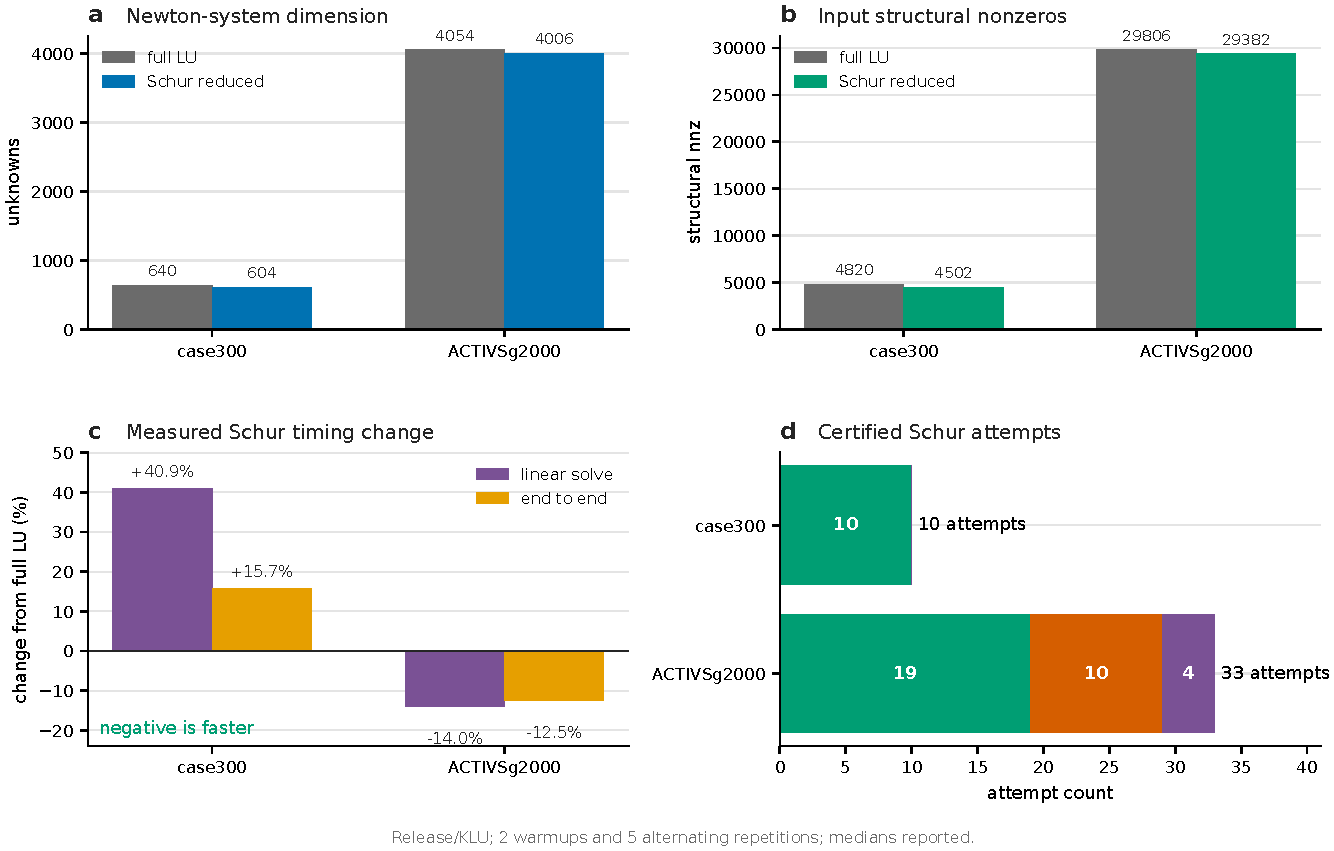
\includegraphics[width=0.94\textwidth]{figures/benchmark_results.pdf}
\caption{Production CPU/KLU Schur benchmark using the fixed two-warmup,
five-repeat alternating protocol. (a) Full and reduced Newton dimensions.
(b) Input structural nonzeros; factor-fill statistics are unavailable from the
current adapter and are not inferred. (c) Median timing change relative to
complete sparse LU, where negative values indicate acceleration. (d) Accepted
and rejected Schur attempts: green denotes accepted steps, orange denotes
local-regularity rejection, and purple denotes reconstructed full-step
backward-error rejection. case300 is a forced research ablation; the production
admission rule excludes it.}
\label{fig:benchmark-results}
\end{figure*}

Figure~\ref{fig:benchmark-results}(a)--(b) confirms the structural predictions: six
states are removed per VSC, and the observed structural reductions exceed the
$48m$ lower bound. It also demonstrates why structure preservation must be
measured rather than assumed. On case300, local factorization and certificate
overhead dominate the small network factorization, so forced Schur is slower.
On ACTIVSg2000, the reduced factorization is large enough to offset the local
work, lowering both linear and end-to-end median time.

The full/Schur median linear and wall times are respectively
$0.491/0.692$~ms and $2.675/3.094$~ms for case300, and
$31.561/27.135$~ms and $47.391/41.486$~ms for ACTIVSg2000. Thus the
visual percentage changes in Fig.~\ref{fig:benchmark-results}(c) retain their
underlying absolute measurements without requiring a duplicate wide table.

For case300, all ten Schur attempts are accepted. The minimum accepted local
$rcond$ is $5.48\times10^{-2}$ and the maximum accepted full backward error is
$3.63\times10^{-17}$. For ACTIVSg2000, 19 of 33 Schur attempts are accepted;
ten are rejected by the local-regularity guard and four by the reconstructed
full backward-error guard. The minimum accepted local $rcond$ is
$2.19\times10^{-8}$, and the maximum accepted full backward error is
$5.96\times10^{-17}$. Rejected attempts use the complete sparse-LU path rather
than terminating the nonlinear solve.

\subsection{Interpretation and present limitations}

The preliminary evidence supports three current claims: the explicit NCP
model remains structurally fixed across activation; the local Schur solve is
algebraically equivalent when its certificate is accepted; and a measurable
CPU benefit appears on the tested 2000-bus hybrid case. The evidence does not
yet support a universal crossover dimension, GPU acceleration, sparse-factor
fill reduction, or large-scale simultaneous binding GFM behavior. The default
dimension of 1000 is therefore exposed as configurable policy and is not
treated as a theorem.

The large GFM datasets currently add one nonbinding Norton GFM block to a
certified MTDC operating point through continuation. They verify data/model
integration and fixed structure, but not flat-start robustness or simultaneous
large-scale GFM limiting. Likewise, weak-grid cases exercise difficult local
roots but do not replace a systematic CPF continuation toward a voltage-
stability nose. These experiments define the remaining work needed before the
results section is submission complete.


\section{Current Scope and Next Experimental Closures}
The present manuscript establishes the balanced positive-sequence model and
the CPU sparse-solver contribution. It does not claim GPU assembly or GPU
factorization. The large hybrid benchmarks contain simultaneous binding
power-port converters, whereas their added large-scale GFM blocks are
currently nonbinding continuation cases. A complete active-mode enumeration
oracle, systematic continuation to the voltage-stability nose, and independent
external selection of the binding GFM priority mode remain required before the
experimental section is considered final. Balanced OPF currently preserves
the authored GFM mode and certifies its dispatch by post-OPF power-flow replay;
the priority NCP is not yet embedded in the OPF KKT system.

\bibliographystyle{IEEEtran}
\bibliography{references}

\end{document}
